% Figure 3.2: SCORM 1.2 CAM Manifest XML Structure
\begin{figure}[htbp]
\centering
\begin{chapterfigurebox}
\begin{tikzpicture}[
    level 1/.style={sibling distance=4.2cm, level distance=1.45cm},
    level 2/.style={sibling distance=2.8cm, level distance=1.35cm},
    level 3/.style={sibling distance=2.1cm, level distance=1.25cm},
    every node/.style={font=\footnotesize, align=center},
    root/.style={rectangle, draw=red!70!black, fill=red!15, thick, minimum width=2.5cm, minimum height=0.8cm, font=\small\bfseries},
    category/.style={rectangle, draw=blue!60!black, fill=blue!10, thick, minimum width=2.3cm, minimum height=0.75cm},
    element/.style={rectangle, draw=green!60!black, fill=green!10, minimum width=2.1cm, minimum height=0.65cm},
    subelement/.style={rectangle, draw=orange!60!black, fill=orange!10, minimum width=1.9cm, minimum height=0.55cm}
]

\node[root] (manifest) {\texttt{<\ENG{manifest}>}}
    [edge from parent fork down]
    child {
        node[category] (metadata) {\texttt{<\ENG{metadata}>}}
        child { node[element] {\texttt{<\ENG{schema}>}} }
        child { node[element] {\texttt{<\ENG{schemaversion}>}} }
        child { node[element] {\texttt{<\ENG{lom}>}} }
    }
    child {
        node[category] (organizations) {\texttt{<\ENG{organizations}>}}
        child {
            node[element] (organization) {\texttt{<\ENG{organization}>}}
            child {
                node[subelement] (item) {\texttt{<\ENG{item}>}}
            }
        }
    }
    child {
        node[category] (resources) {\texttt{<\ENG{resources}>}}
        child {
            node[element] (resource) {\texttt{<\ENG{resource}>}}
            child {
                node[subelement] (file) {\texttt{<\ENG{file}>}}
            }
        }
    };

% Attribute notes
\node[font=\tiny, anchor=west, text=gray] at ([xshift=0.25cm]organizations.east)
{@\ENG{default}};

\node[font=\tiny, anchor=west, text=gray] at ([xshift=0.25cm]organization.east)
{@\ENG{identifier}};

\node[font=\tiny, anchor=west, align=left, text=gray] at ([xshift=0.25cm]item.east)
{@\ENG{identifier},\\ @\ENG{identifierref}};

\node[font=\tiny, anchor=west, align=left, text=gray] at ([xshift=0.25cm]resource.east)
{@\ENG{identifier},\\ @\ENG{type}, @\ENG{href}};

\end{tikzpicture}
\end{chapterfigurebox}
\medskip
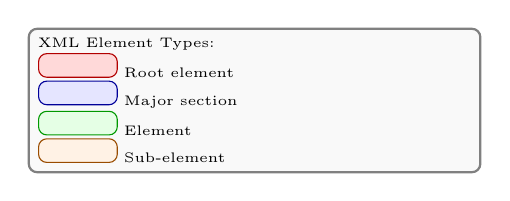
\begin{tikzpicture}
\node[draw=black!50, fill=gray!5, thick, rounded corners=3pt,
      align=left, font=\tiny, text width=5.5cm] {
\ENG{XML Element Types}:\\
\tikz{\node[rectangle, draw=red!70!black, fill=red!15, minimum width=1cm, minimum height=0.3cm] {};} Root element \\
\tikz{\node[rectangle, draw=blue!60!black, fill=blue!10, minimum width=1cm, minimum height=0.3cm] {};} Major section \\
\tikz{\node[rectangle, draw=green!60!black, fill=green!10, minimum width=1cm, minimum height=0.3cm] {};} Element \\
\tikz{\node[rectangle, draw=orange!60!black, fill=orange!10, minimum width=1cm, minimum height=0.3cm] {};} Sub-element
};
\end{tikzpicture}
\caption{Ιεραρχική δομή του \ENG{imsmanifest.xml}. Το \ENG{root} element \texttt{<\ENG{manifest}>} περιέχει τις ενότητες \texttt{<\ENG{metadata}>}, \texttt{<\ENG{organizations}>} και \texttt{<\ENG{resources}>}.}
\label{fig:scorm12_cam_manifest_structure}
\end{figure}
